\section{Experiments}


\subsection{Setup}~\label{sec: exp_setup}
\vspace{-5mm}

Following existing work~\citep{wang2025agent}, we conduct experiments on WebArena~\citep{zhou2024webarena} which features general web navigation across diverse domains\footnote{We exclude the domain of \textit{Map} due to website issues following~\cite{miyai2025webchorearena} for a fair comparison.}, and Mind2Web~\citep{deng2023mind2web} that tests generalization of agents on versatile operations and environments. We also conduct experiment on SWE-Bench-Verified for repository-level issue-resolving.
For comparison, we consider baselines ranging from memory-free agents (No Memory) to trajectory-based memory (Synapse)~\citep{zheng2024synapse} and workflow-based memory (AWM)~\citep{wang2025agent}.
Our agents are built on Gemini-2.5~\citep{comanici2025gemini} and Claude-3.7~\citep{Anthropic} models using BrowserGym~\citep{chezelles2025browsergym} for web browsing and bash-only for SWE, following ReAct~\citep{yao2023react} style with default decoding configurations.
We evaluate effectiveness (success rate, SR) and efficiency (average steps, AS), with specific metrics varying for each dataset. 
Full descriptions for datasets, baselines, implementations, and evaluation are in Appendix~\ref{app: exp_setting_detail}.

\begin{table}[t]
\centering\setlength{\tabcolsep}{5.3pt}
\small
\setlength{\belowcaptionskip}{6.0pt}
  \caption{Experiment results of \ours{} and \mats{} (parallel scaling, $k=5$, pass@1) on WebArena benchmark. Success rate (SR $\uparrow$) and the number of steps (Step $\downarrow$) are reported on 5 subsets for 3 different backbone LLMs.}
  \label{table: webarena}
  \begin{tabular}{lcccccccccccc}
    \toprule
    \multirow{2}{*}{\textbf{Models}} &\multicolumn{2}{c}{\textbf{Shopping}}&\multicolumn{2}{c}{\textbf{Admin}}&\multicolumn{2}{c}{\textbf{Gitlab}}&\multicolumn{2}{c}{\textbf{Reddit}}&\multicolumn{2}{c}{\textbf{Multi}}&\multicolumn{2}{c}{\textbf{\underline{Overall}}}\\
    &\multicolumn{2}{c}{(187)}&\multicolumn{2}{c}{(182)} &\multicolumn{2}{c}{(180)} & \multicolumn{2}{c}{(106)}&\multicolumn{2}{c}{(29)}&\multicolumn{2}{c}{(684)}\\
\cmidrule(lr){2-3}\cmidrule(lr){4-5}\cmidrule(lr){6-7}\cmidrule(lr){8-9}\cmidrule(lr){10-11}\cmidrule(lr){12-13}
&\textit{SR}&\textit{Step}&\textit{SR}&\textit{Step}&\textit{SR}&\textit{Step}&\textit{SR}&\textit{Step}&\textit{SR}&\textit{Step}&\textit{SR}&\textit{Step} \\
    \midrule
    \multicolumn{13}{c}{\cellcolor{gray!15}\textit{Gemini-2.5-flash}} \\
    No Memory &39.0&8.2&44.5&9.5&33.9&13.3&55.7&6.7&10.3&10.0&40.5&9.7\\
    Synapse&40.6&7.0&45.1&9.1&35.6&13.0&59.4&6.5&10.3&10.5&42.1&9.2\\
    AWM&44.4&7.0&46.7&8.8&37.2&13.2&62.3&6.1&3.4&\textbf{7.7}&44.1&9.0\\
    \hdashline
    \ours{} &\textbf{49.7}&\textbf{6.1}&\textbf{51.1}&\textbf{8.2}&\textbf{40.6}&\textbf{12.3}&\textbf{67.0}&\textbf{5.6}&\textbf{13.8}&8.8&\textbf{48.8}&\textbf{8.3} \\
    \dab{+\mats{}} &53.0 & 6.3&53.8&7.6&42.8&11.9&70.8&5.4&17.2&8.0 &51.8&7.9\\
    \midrule
    \multicolumn{13}{c}{\cellcolor{gray!15}\textit{Gemini-2.5-pro}} \\
    No Memory&45.5&7.6&51.1&8.7&35.0&11.6&71.7&6.0&6.9&8.8&46.7&8.8\\
    Synapse&46.5&6.6&52.2&8.9&38.3&11.3&68.9&5.9&6.9&9.0&47.7&8.5\\
    AWM&48.1&6.4&49.3&9.8&40.0&11.2&68.9&6.4&3.4&9.3&47.6&8.7\\
    \hdashline
    \ours{} & \textbf{51.9}&\textbf{6.0}&\textbf{56.6}&\textbf{7.7}&\textbf{44.4}&\textbf{9.8}&\textbf{80.2}&\textbf{5.1}&\textbf{13.8}&\textbf{8.2}&\textbf{53.9}&\textbf{7.4}\\
    \dab{+\mats{}} &54.0 & 5.9&58.2&7.4&46.7&9.1&83.0&5.3&20.7&7.2&56.3&7.1\\
    \midrule
    \multicolumn{13}{c}{\cellcolor{gray!15}\textit{Claude-3.7-sonnet}} \\
    No Memory&38.5&6.1&49.5&8.4&36.7&10.6&53.8&5.5&0.0&11.6&41.7&8.0\\
    Synapse&39.6&5.8&50.5&8.5&38.0&10.0&53.8&6.1&0.0&11.8&42.6&7.9\\
    AWM&39.6&7.2&47.8&9.3&34.6&10.9&52.8&7.0&0.0&12.4&40.8&8.9\\
    \hdashline
    \ours{} &\textbf{44.9}&\textbf{5.6}&\textbf{53.3}&\textbf{7.6}&\textbf{41.1}&\textbf{9.5}&\textbf{57.5}&\textbf{5.2}&\textbf{3.4}&\textbf{10.5}&\textbf{46.3}&\textbf{7.3} \\
    \dab{+\mats{}} &47.1&5.8&55.5&7.4&43.3&9.4&60.4&5.0&10.3&9.1&48.8&7.2\\

  \bottomrule
\end{tabular}
\vspace{-5mm}
\end{table}

\subsection{Results of \ours{}}

Tables \ref{table: webarena}, \ref{table: mind2web}, \ref{table: swebench} summarize the main evaluation results of \ours{} on WebArena, Mind2Web, and SWE-Bench-Verified accordingly. We have the following observations.

\noindent\textbf{\ours{} consistently outperforms baselines across LLM backbones on all datasets.}
Specifically, \ours{} improves the overall success rate on WebArena (Table~\ref{table: webarena}) by $+8.3$, $+7.2$, and $+4.6$ with three different backbone LLMs compared to memory-free agents. A similar pattern holds on Mind2Web (Table~\ref{table: mind2web}), where \ours{} delivers clear gains across cross-task, cross-website, and cross-domain settings, underscoring both the consistency and scalability of its benefits across datasets and model sizes. Results on SWE-Bench-Verified (Table~\ref{table: swebench}) further confirm its robustness. 
Crucially, unlike baselines such as Synapse and AWM that rely on a narrow, homogeneous memory source derived exclusively from successful trajectories, \ours{} employs a superior extraction strategy that is key to its consistent out-performance.

\begin{wraptable}{t}{0.4\textwidth}
\vspace{-5mm}
\centering\setlength{\tabcolsep}{4pt}
\small
\setlength{\belowcaptionskip}{1pt}
  \caption{Experiment results of \ours{} on SWE-Bench-Verified dataset for issue-resolving in a given repository.}
  \label{table: swebench}
  \begin{tabular}{lcc}
    \toprule
    Methods & Resolve Rate & AS\\
    \midrule
    \multicolumn{3}{c}{\cellcolor{gray!15}\textit{Gemini-2.5-flash}}\\
    No Memory & 34.2&30.3\\
    Synapse& 35.4&30.7\\
    \ours{} & \textbf{38.8}& \textbf{27.5}\\
    \midrule
    \multicolumn{3}{c}{\cellcolor{gray!15}\textit{Gemini-2.5-pro}} \\
    No Memory&54.0&21.1\\
    Synapse&53.4&21.0 \\
    \ours{} & \textbf{57.4}&\textbf{19.8}\\
  \bottomrule
\end{tabular}
\vspace{-3mm}
\end{wraptable}

\noindent\textbf{\ours{} enhances generalization with better transferrable memory across tasks.} 
We also evaluate in challenging generalization settings. On WebArena (Table~\ref{table: webarena}), the \textit{Multi} subset requires transferring memory across multiple websites, where \ours{} achieves a notable gain of $+4.6$ averaged SR over the strongest baseline. In contrast, strong baselines such as AWM fail to provide gains and even degrade in this setting. On Mind2Web (Table~\ref{table: mind2web}), which includes cross-task, cross-website, and cross-domain evaluations that impose progressively higher demands, \ours{} consistently improves success rates. The gains are especially pronounced in the cross-domain setting, which requires the highest level of generalization. These results demonstrate that memory curated by \ours{} is more robust and transferable, enabling agents to generalize effectively across diverse scenarios.

\begin{table}[!t]
\centering\setlength{\tabcolsep}{5.3pt}
\small
\setlength{\belowcaptionskip}{1pt}
  \caption{Results on Mind2Web benchmark for cross-task, cross-website, and cross-domain generalization test. EA ($\uparrow$) is short for element accuracy, AF$_1$ ($\uparrow$) is short for action F$_1$, and SSR ($\uparrow$) is short for step success rate. SR ($\uparrow$) is the task-level success rate measuring if all steps are correct. }
  \label{table: mind2web}
  \begin{tabular}{lcccccccccccc}
    \toprule
    \multirow{2}{*}{\textbf{Models}} &\multicolumn{4}{c}{\textbf{Cross-Task}}&\multicolumn{4}{c}{\textbf{Cross-Website}}&\multicolumn{4}{c}{\textbf{Cross-Domain}}\\
\cmidrule(lr){2-5}\cmidrule(lr){6-9}\cmidrule(lr){10-13}
&\textit{EA}&\textit{AF$_1$}&\textit{SSR}&\textit{SR}&\textit{EA}&\textit{AF$_1$}&\textit{ SSR}&\textit{SR}&\textit{EA}&\textit{AF$_1$}&\textit{SSR}&\textit{SR} \\
    \midrule
    \multicolumn{13}{c}{\cellcolor{gray!15}\textit{Gemini-2.5-flash}} \\
    No Memory &46.0&59.1&40.3&3.3&39.8&45.1&31.7&1.7&35.8&37.9&31.9&1.0 \\
    Synapse&47.0&59.5&41.2&3.5&40.3&46.0&32.1&1.9&36.3&38.5&32.4&1.1 \\
    AWM & 46.3&56.1&41.0&3.5&39.1&42.2&31.7&2.1&33.3&36.5&30.1&0.7\\
    \ours{} & \textbf{52.1}&\textbf{60.4}&\textbf{44.9}&\textbf{4.8}&\textbf{44.3}&\textbf{52.6}&\textbf{33.9}&\textbf{2.3}&\textbf{40.6}&\textbf{41.3}&\textbf{36.6}&\textbf{1.6}  \\
    \midrule
    \multicolumn{13}{c}{\cellcolor{gray!15}\textit{Gemini-2.5-pro}} \\
    No Memory&49.3&60.2&44.4&3.5&41.2&49.8&34.8&3.4&37.9&37.7&35.0&1.4\\
    Synapse&50.1&61.0&44.7&3.6&41.8&51.2&35.0&3.2&38.5&39.8&35.6&1.5\\
    AWM&48.6&61.2&44.4&3.7&41.9&47.9&34.8&2.3&37.3&38.1&34.4&1.2\\
    \ours{} &\textbf{53.6}&\textbf{62.7}&\textbf{45.6}&\textbf{5.1}&\textbf{46.1}&\textbf{54.8}&\textbf{36.9}&\textbf{3.8}&\textbf{42.8}&\textbf{45.2}&\textbf{38.1}&\textbf{1.7} \\

  \bottomrule
\end{tabular}
\vspace{-5mm}
\end{table}



\noindent\textbf{\ours{} achieves superior efficiency by leveraging past experiences as memory.}
In addition to higher success rates, \ours{} also reduces the number of interaction steps needed to complete tasks, as shown in the \textit{Step} metric of Table~\ref{table: webarena} and \ref{table: swebench}. On WebArena, across almost all subsets and backbones, \ours{} lowers the average step count by up to $1.4$ compared with ``No Memory'', and $1.6$ compared with other memory baselines. The average step on SWE-Bench-Verified is also smaller by saving $2.8$ and $1.3$ steps respectively. This indicates that \ours{} enables agents to solve tasks more efficiently by reusing and refining reasoning knowledge, thus avoiding unnecessary or redundant exploration.




\subsection{Results of \mats{}}\label{sec: res_mats}


We first present the overall results of \mats{} on WebArena in Table~\ref{table: webarena}, which demonstrate additional strong performance improvement and efficiency gains with \ours{}.\footnote{By default, \mats{} integrates \ours{}, but it could also use other memory mechanisms.} To study the scaling effect in-depth with both parallel and sequential variants, we experimented \mats{} with Gemini-2.5-flash on Webarena-Shopping subset. To investigate the overall scaling effect, we benchmark with \textbf{(i) \mats{} w/o memory}, which represents the scaling setting without memory mechanism, \textbf{(ii) \mats{} w/o aggregation}, which is equal to Vanilla TTS in Figure~\ref{fig: mats}(a) and \textbf{(iii) \mats{}} to demonstrate the effect with respect to scaling factor $k$. Notably, $k=1$ is the setting without scaling. For parallel scaling, we compute Best-of-N (BoN) as the final metric detailed in Appendix~\ref{app: prompt_mats}. Results are shown in Figure~\ref{fig: scaling_mats}.


\noindent\textbf{Both parallel scaling and sequential scaling boost performance.}
Increasing $k$ generally improves success rate, confirming the benefit of allocating more inference-time computation. With \mats{}, parallel scaling grows from $49.7$ ($k=1$) to $55.1$ ($k=5$), while sequential scaling rises from $49.7$ to $54.5$. For the baseline of \mats{} w/o memory, the gains are smaller and less consistent (e.g., parallel scaling fluctuates between $39.0$ and $42.2$ and sequential scaling fluctuates between $37.4$ and $40.6$). In contrast, \mats{} enables stronger and more stable improvements across both scaling strategies, highlighting its role in making scaling more effective.

\noindent\textbf{\mats{} is consistently better than vanilla TTS.}
With \ours{}, \mats{} consistently surpasses \mats{} w/o aggregation (vanilla TTS), showing that memory-aware coordination and aggregation is important. Specifically, at $k=5$, \mats{} achieves $55.1$ in parallel scaling compared with $52.4$ for vanilla TTS, and $54.5$ versus $51.9$ in sequential scaling. These improvements highlight that memory-aware scaling effectively directs the agent toward more promising solutions by synthesizing insights from multiple trajectories or interaction steps to leverage contrastive signals.

\begin{wrapfigure}{r}{0.6\textwidth}
% \vspace{-3mm}
  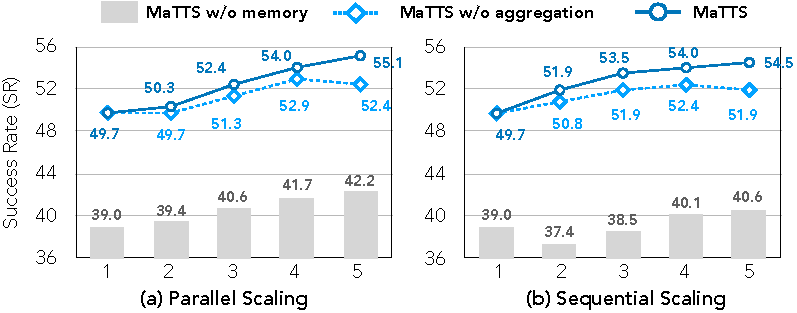
\includegraphics[width=0.6\textwidth]{figures/scaling_mats.pdf}
  \vspace{-5mm}
  \caption{Effect of scaling factor $k$ for \mats{} under with \ours{} on WebArena-Shopping subset. We compare (a) parallel and (b) sequential test-time scaling.}
  \label{fig: scaling_mats}
  \vspace{-3mm}
\end{wrapfigure}

\noindent\textbf{Sequential scaling shows short-term advantage, but parallel dominates at larger scales for \ours{}.}
With stronger memory mechanisms such as \ours{}, sequential refinement brings higher gains at small $k$, but its benefit quickly saturates—once the model either succeeds or fails decisively, further refinements add little new insight. In contrast, parallel scaling continues to provide diverse rollouts that allow the model to critique and improve upon its own generations, leading it to surpass sequential at larger $k$ (e.g., $55.1$ vs. $54.5$ at $k=5$). In contrast, for vanilla TTS which is not equipped with memory module, sequential scaling yields little or even no benefit as scaling goes on, and parallel scaling consistently dominates.


\subsection{Synergy of Memory and Test-Time Scaling}\label{sec: exp_synergy}

While the previous section establishes the overall effectiveness of \mats{}, we highlight the synergy between memory and TTS in this section. Figure~\ref{fig: res_mats} presents a snapshot of \mats{} on the WebArena-Shopping subset with parallel scaling factor $k=5$, where we report both Pass@1 (randomly selected trajectory) and Best-of-5 (BoN). This setting allows us to examine the bidirectional interaction between memory quality and scaling effectiveness.

\begin{wrapfigure}{r}{0.5\textwidth}
% \vspace{-3mm}
  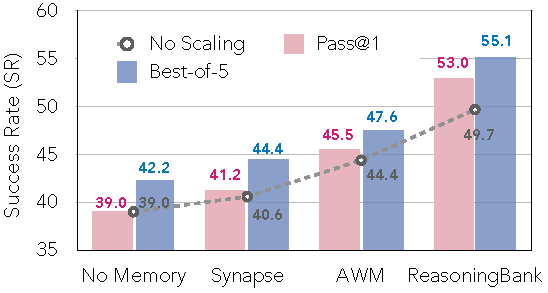
\includegraphics[width=0.5\textwidth]{figures/res_mats.pdf}
  \vspace{-5mm}
  \caption{Snapshot of \mats{} on WebArena-Shopping subset with different memory mechanisms with $k=5$. We compute BoN for all $5$ trajectories and Pass@1 with one randomly selected trajectory.}
  \label{fig: res_mats}
  \vspace{-3mm}
\end{wrapfigure}

\sethlcolor{bluebar}
\noindent\textbf{Better memory enables stronger test-time scaling performance.}
To see how memory improves the effectiveness of scaling, we focus on the BoN results, which directly measure an agent’s ability to surface the best outcome among multiple rollouts. As shown by \hl{blue bars} in Figure~\ref{fig: res_mats}, the benefit of scaling depends critically on the underlying memory. Without memory, scaling yields slight improvement, with BoN rising only from $39.0$ to $42.2$. Weaker memory mechanisms such as Synapse and AWM provide moderate gains, reaching $44.4$ and $47.6$, respectively. In contrast, \mats{} with \ours{} delivers the strongest benefit, with BoN climbing from $49.7$ to $55.1$. These results show that high-quality memory directs scaling toward more promising rollouts, ensuring that the additional trajectories are not wasted but converted into higher success rates.



\sethlcolor{pinkbar}
\noindent\textbf{Scaling yields better memory curation.}
To fairly evaluate how scaling feeds back into memory, we report Pass@1, which measures the average quality of trajectories after memory curation and allows direct comparison with the no-scaling case. The trend is depicted in \hl{pick bars} and is striking: scaling actually reduces performance for weaker memories, where Synapse slightly increases from $40.6$ to $41.2$, and AWM from $44.4$ to $45.5$. These phenomenon suggest that without strong guidance, the extra rollouts generated by scaling offer diminishing returns. In contrast, \ours{} provides far more benefits: Pass@1 rises from $49.7$ to $53.0$, showing that high-quality memory can harness the diversity of scaling to extract constructive contrastive signals. This asymmetry highlights that scaling alone is insufficient; only when paired with good memory mechanism does it contribute to curation of more effective memory, closing the virtuous cycle.


